\documentclass[11pt,a4paper]{report}
\usepackage[textwidth=37em,vmargin=30mm]{geometry}
\usepackage{calc,xunicode,amsmath,amssymb,paralist,enumitem,tabu,booktabs,datetime2,xeCJK,xeCJKfntef,listings}
\usepackage{tocloft,fancyhdr,tcolorbox,xcolor,graphicx,eso-pic,xltxtra,xelatexemoji}

\newcommand{\envyear}[0]{2025}
\newcommand{\envdatestr}[0]{2025-01-16}
\newcommand{\envfinaldir}[0]{webdb/2025/20250116/final}

\usepackage[hidelinks]{hyperref}
\hypersetup{
    colorlinks=false,
    pdfpagemode=FullScreen,
    pdftitle={Web Digest - \envdatestr}
}

\setlength{\cftbeforechapskip}{10pt}
\renewcommand{\cftchapfont}{\rmfamily\bfseries\large\raggedright}
\setlength{\cftbeforesecskip}{2pt}
\renewcommand{\cftsecfont}{\sffamily\small\raggedright}

\setdefaultleftmargin{2em}{2em}{1em}{1em}{1em}{1em}

\usepackage{xeCJK,xeCJKfntef}
\xeCJKsetup{PunctStyle=plain,RubberPunctSkip=false,CJKglue=\strut\hskip 0pt plus 0.1em minus 0.05em,CJKecglue=\strut\hskip 0.22em plus 0.2em}
\XeTeXlinebreaklocale "zh"
\XeTeXlinebreakskip = 0pt


\setmainfont{Brygada 1918}
\setromanfont{Brygada 1918}
\setsansfont{IBM Plex Sans}
\setmonofont{JetBrains Mono NL}
\setCJKmainfont{Noto Serif CJK SC}
\setCJKromanfont{Noto Serif CJK SC}
\setCJKsansfont{Noto Sans CJK SC}
\setCJKmonofont{Noto Sans CJK SC}

\setlength{\parindent}{0pt}
\setlength{\parskip}{8pt}
\linespread{1.15}

\lstset{
	basicstyle=\ttfamily\footnotesize,
	numbersep=5pt,
	backgroundcolor=\color{black!5},
	showspaces=false,
	showstringspaces=false,
	showtabs=false,
	tabsize=2,
	captionpos=b,
	breaklines=true,
	breakatwhitespace=true,
	breakautoindent=true,
	linewidth=\textwidth
}






\newcommand{\coverpic}[2]{
    % argv: itemurl, authorname
    Cover photo by #2~~(\href{#1}{#1})
}
\newcommand{\makeheader}[0]{
    \begin{titlepage}
        % \newgeometry{hmargin=15mm,tmargin=21mm,bmargin=12mm}
        \begin{center}
            
            \rmfamily\scshape
            \fontspec{BaskervilleF}
            \fontspec{Old Standard}
            \fontsize{59pt}{70pt}\selectfont
            WEB\hfill DIGEST
            
            \vfill
            % \vskip 30pt
            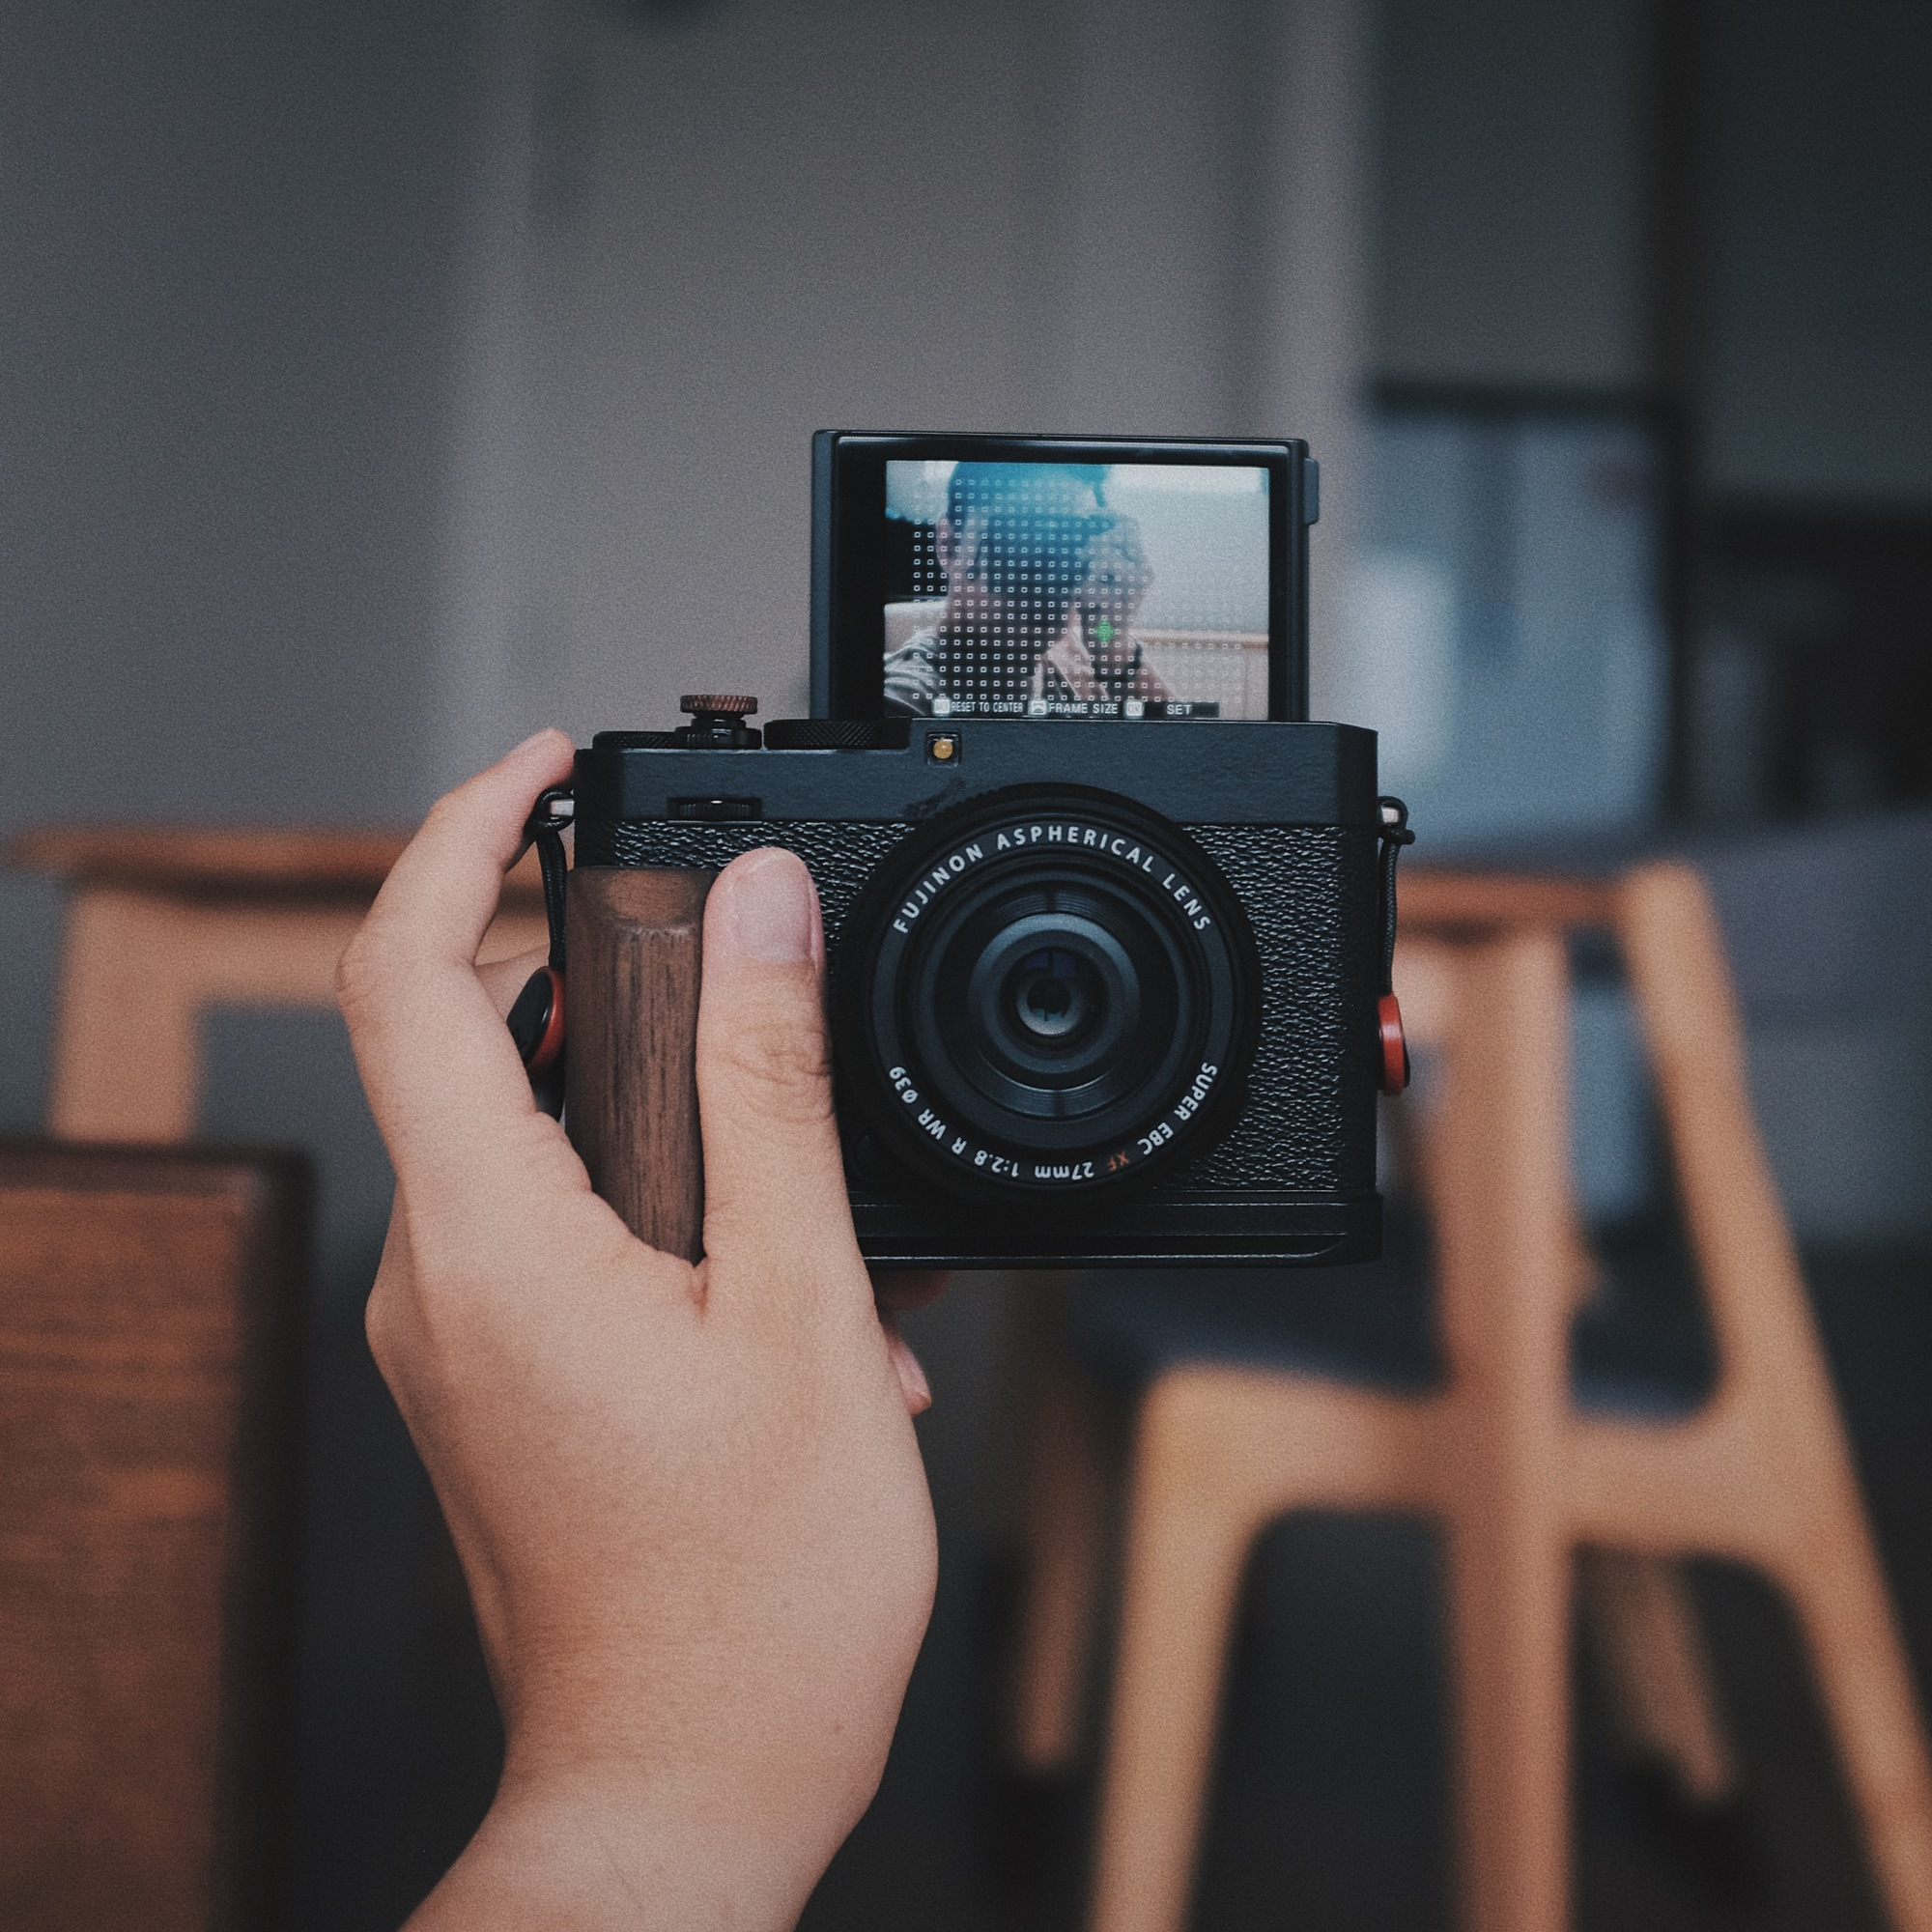
\includegraphics[width=\linewidth]{\envfinaldir/coverpic-prod.jpg}\par
            % \vskip 30pt
            \vfill

            \normalsize\rmfamily\scshape
            \copyright{} The Web Digest Project \hfill\large \envdatestr
        \end{center}
    \end{titlepage}
    % \restoregeometry
}
\newcommand{\simplehref}[1]{%
    \textcolor{blue!80!green}{\href{#1}{#1}}%
}
\renewcommand{\contentsname}{\center\Huge\sffamily\bfseries Contents\par\vskip 20pt}
\newcounter{ipartcounter}
\setcounter{ipartcounter}{0}
\newcommand{\ipart}[1]{
    % \vskip 20pt
    \clearpage
    \stepcounter{ipartcounter}
    \phantomsection
    \addcontentsline{toc}{chapter}{#1}
    % \begin{center}
    %     \Huge
    %     \sffamily\bfseries
    %     #1
    % \end{center}
    % \vskip 20pt plus 7pt
}
\newcounter{ichaptercounter}
\setcounter{ichaptercounter}{0}
\newcommand{\ichapter}[1]{
    % \vskip 20pt
    \clearpage
    \stepcounter{ichaptercounter}
    \phantomsection
    \addcontentsline{toc}{section}{\numberline{\arabic{ichaptercounter}}#1}
    \begin{center}
        \Huge
        \sffamily\bfseries
        #1
    \end{center}
    \vskip 20pt plus 7pt
}
\newcommand{\entrytitlefont}[1]{\subsection*{\raggedright\Large\sffamily\bfseries#1}}
\newcommand{\entryitemGeneric}[2]{
    % argv: title, url
    \parbox{\linewidth}{
        \entrytitlefont{#1}\par\vskip 5pt
        \footnotesize\ttfamily\mdseries
        \simplehref{#2}
    }\vskip 11pt plus 11pt minus 1pt
}
\newcommand{\entryitemGithub}[3]{
    % argv: title, url, desc
    \parbox{\linewidth}{
        \entrytitlefont{#1}\par\vskip 5pt
        \footnotesize\ttfamily\mdseries
        \simplehref{#2}\par\vskip 5pt
        \small\rmfamily\mdseries#3
    }\vskip 11pt plus 11pt minus 1pt
}
\newcommand{\entryitemAp}[3]{
    % argv: title, url, desc
    \parbox{\linewidth}{
        \entrytitlefont{#1}\par\vskip 5pt
        \footnotesize\ttfamily\mdseries
        \simplehref{#2}\par\vskip 5pt
        \small\rmfamily\mdseries#3
    }\vskip 11pt plus 11pt minus 1pt
}
\newcommand{\entryitemHackernews}[3]{
    % argv: title, hnurl, rawurl
    % \parbox{\linewidth}{
    %     \entrytitlefont{#1}\par\vskip 5pt
    %     \footnotesize\ttfamily\mdseries
    %     \simplehref{#3}\par
    %     \textcolor{black!50}{\href{#2}{#2}}
    % }\vskip 11pt plus 11pt minus 1pt
    \begin{minipage}{\linewidth}
            \entrytitlefont{#1}\par\vskip 5pt
            \footnotesize\ttfamily\mdseries
            \simplehref{#3}\par
            \textcolor{black!50}{\href{#2}{#2}}
    \end{minipage}\par\vskip 11pt plus 11pt minus 1pt
}







\begin{document}

\makeheader

\tableofcontents\clearpage




\ipart{Developers}
\ichapter{Hacker News}
\entryitemTwoLinks{I have made the decision to disband Hindenburg Research}{https://news.ycombinator.com/item?id=42717234}{https://hindenburgresearch.com/gratitude/}

\entryitemTwoLinks{UnitedHealth overcharged cancer patients for drugs by over 1,000\%}{https://news.ycombinator.com/item?id=42716428}{https://fortune.com/2025/01/15/ftc-pbms-unitedhealth-brian-thompson-cvs-caremark-cigna-pharmacy-benefit-managers/}

\entryitemTwoLinks{Sweden brings more books and handwriting practice back to its schools (2023)}{https://news.ycombinator.com/item?id=42715841}{https://apnews.com/article/sweden-digital-education-backlash-reading-writing-1dd964c628f76361c43dbf3964f7dbf4}

\entryitemTwoLinks{A marriage proposal spoken in office jargon}{https://news.ycombinator.com/item?id=42714775}{https://www.mcsweeneys.net/articles/a-marriage-proposal-spoken-entirely-in-office-jargon}

\entryitemTwoLinks{Qantas South Africa flights delayed by falling debris from SpaceX rockets}{https://news.ycombinator.com/item?id=42714436}{https://www.theguardian.com/business/2025/jan/14/qantas-flights-delayed-spacex-falling-debris-sydney-to-johannesburg}

\entryitemTwoLinks{GOG Joins European Federation of Game Archives, Museums \& Preservation Projects}{https://news.ycombinator.com/item?id=42714156}{https://www.gamingonlinux.com/2025/01/gog-joins-the-european-federation-of-game-archives-museums-and-preservation-projects/}

\entryitemTwoLinks{Why is Cloudflare Pages' bandwidth unlimited?}{https://news.ycombinator.com/item?id=42712433}{https://mattsayar.com/why-does-cloudflare-pages-have-such-a-generous-free-tier/}

\entryitemTwoLinks{Ropey – A UTF8 text rope for manipulating and editing large text}{https://news.ycombinator.com/item?id=42711966}{https://github.com/cessen/ropey}

\entryitemTwoLinks{WTF Happened in 1971? (2019)}{https://news.ycombinator.com/item?id=42711781}{https://wtfhappenedin1971.com/}

\entryitemTwoLinks{Norepinephrine-mediated slow vasomotion drives glymphatic clearance during sleep}{https://news.ycombinator.com/item?id=42711751}{https://www.cell.com/cell/abstract/S0092-8674(24)01343-6}

\entryitemTwoLinks{Build a Database in Four Months with Rust and 647 Open-Source Dependencies}{https://news.ycombinator.com/item?id=42711727}{https://tisonkun.io/posts/oss-twin}

\entryitemTwoLinks{US will ban cancer-linked Red Dye No. 3 in cereal and other foods}{https://news.ycombinator.com/item?id=42711556}{https://www.bloomberg.com/news/articles/2025-01-15/us-fda-to-ban-red-dye-no-3-rfk-went-after-due-to-cancer-link}

\entryitemTwoLinks{Modern JavaScript for Django developers}{https://news.ycombinator.com/item?id=42711387}{https://www.saaspegasus.com/guides/modern-javascript-for-django-developers/}

\entryitemTwoLinks{Google is making AI in Gmail and Docs free, but raising the price of Workspace}{https://news.ycombinator.com/item?id=42710978}{https://www.theverge.com/2025/1/15/24343794/google-workspace-ai-features-free}

\entryitemTwoLinks{TikTok preparing for U.S. shut-off on Sunday}{https://news.ycombinator.com/item?id=42710339}{https://www.reuters.com/technology/tiktok-preparing-us-shut-off-sunday-information-reports-2025-01-15/}

\entryitemTwoLinks{Sky-scanning complete for Gaia}{https://news.ycombinator.com/item?id=42709105}{https://www.esa.int/ESA\_Multimedia/Images/2025/01/Sky-scanning\_complete\_for\_Gaia}

\entryitemTwoLinks{Generate audiobooks from E-books with Kokoro-82M}{https://news.ycombinator.com/item?id=42708773}{https://claudio.uk/posts/epub-to-audiobook.html}

\entryitemTwoLinks{Nevada court shuts down police use of federal loophole for civil forfeiture}{https://news.ycombinator.com/item?id=42707573}{https://ij.org/press-release/nevada-court-shuts-down-police-use-of-federal-loophole-for-civil-forfeiture/}

\entryitemTwoLinks{Nobody cares}{https://news.ycombinator.com/item?id=42707238}{https://grantslatton.com/nobody-cares}

\entryitemTwoLinks{Rsync vulnerabilities}{https://news.ycombinator.com/item?id=42706732}{https://www.openwall.com/lists/oss-security/2025/01/14/3}\ichapter{Phoronix}
\entryitemGeneric{\hskip 0pt{}Tiny Corp Nearing "Completely Sovereign" Compute Stack For AMD GPUs With Tinygrad}{https://www.phoronix.com/news/Tiny-Sovereign-Stack-AMD-Close}

\entryitemGeneric{\hskip 0pt{}Intel THC Drivers To Be Submitted For Linux 6.14}{https://www.phoronix.com/news/Intel-THC-For-Linux-6.14}

\entryitemGeneric{\hskip 0pt{}NVMe PCI Endpoint Function Target Driver Coming To Linux 6.14}{https://www.phoronix.com/news/Linux-6.14-PCIe-NVMe-Target-EPF}

\entryitemGeneric{\hskip 0pt{}Triple Buffering Support Updated Against Latest GNOME 48 Code}{https://www.phoronix.com/news/GNOME-48-Triple-Buffering-Jan}

\entryitemGeneric{\hskip 0pt{}Linux 6.14 To Bring An Important Improvement For AMD Preferred Core}{https://www.phoronix.com/news/AMD-Preferred-Core-Better-6.14}

\entryitemGeneric{\hskip 0pt{}Xen Hypervisor Support Being Worked On For RISC-V}{https://www.phoronix.com/news/Xen-RISC-V-Linux-Patches}

\entryitemGeneric{\hskip 0pt{}libvirt 11.0 Released For Open-Source Virtualization API}{https://www.phoronix.com/news/libvirt-11.0}

\entryitemGeneric{\hskip 0pt{}LACT Linux GPU Control Panel Adds Support For Intel Graphics}{https://www.phoronix.com/news/LACT-0.7-GPU-Control-Panel}

\entryitemGeneric{\hskip 0pt{}Intel "Performance Tips" Published For Optimal Linux Graphics}{https://www.phoronix.com/news/Intel-Perf-Tips-Linux-Graphics}\ichapter{Dribbble}
\entryitemGeneric{\hskip 0pt{}Puzzle Fintech Website Design}{https://dribbble.com/shots/25394559-Puzzle-Fintech-Website-Design}

\entryitemGeneric{\hskip 0pt{}Black Cats}{https://dribbble.com/shots/25478711-Black-Cats}

\entryitemGeneric{\hskip 0pt{}RoundRobin 2.0}{https://dribbble.com/shots/25479558-RoundRobin-2-0}

\entryitemGeneric{\hskip 0pt{}Gillespie Farms™}{https://dribbble.com/shots/25474556-Gillespie-Farms}

\entryitemGeneric{\hskip 0pt{}Faith Education Icons}{https://dribbble.com/shots/25422138-Faith-Education-Icons}

\entryitemGeneric{\hskip 0pt{}Round Robin}{https://dribbble.com/shots/25467606-Round-Robin}

\entryitemGeneric{\hskip 0pt{}Kraken Illustration}{https://dribbble.com/shots/25468020-Kraken-Illustration}

\entryitemGeneric{\hskip 0pt{}Nexos crypto wallet}{https://dribbble.com/shots/25464532-Nexos-crypto-wallet}

\entryitemGeneric{\hskip 0pt{}Document Scanner App}{https://dribbble.com/shots/25466972-Document-Scanner-App}

\entryitemGeneric{\hskip 0pt{}Pythagoras}{https://dribbble.com/shots/25467709-Pythagoras}

\entryitemGeneric{\hskip 0pt{}The best route to the corner office}{https://dribbble.com/shots/25468475-The-best-route-to-the-corner-office}

\entryitemGeneric{\hskip 0pt{}Learning App Design}{https://dribbble.com/shots/25458950-Learning-App-Design}

\entryitemGeneric{\hskip 0pt{}Cub Studio Process}{https://dribbble.com/shots/25456521-Cub-Studio-Process}

\entryitemGeneric{\hskip 0pt{}Southland Provisions}{https://dribbble.com/shots/25456279-Southland-Provisions}

\entryitemGeneric{\hskip 0pt{}Polar Bear + Baby (2012)}{https://dribbble.com/shots/25454483-Polar-Bear-Baby-2012}

\entryitemGeneric{\hskip 0pt{}SHOWREEL 24'}{https://dribbble.com/shots/25450148-SHOWREEL-24}

\entryitemGeneric{\hskip 0pt{}Yacht Life}{https://dribbble.com/shots/25456479-Yacht-Life}

\entryitemGeneric{\hskip 0pt{}Cromatic.bio®}{https://dribbble.com/shots/25451539-Cromatic-bio}

\entryitemGeneric{\hskip 0pt{}Running Dog Logo}{https://dribbble.com/shots/25450403-Running-Dog-Logo}

\entryitemGeneric{\hskip 0pt{}REV Graphic Style}{https://dribbble.com/shots/25452261-REV-Graphic-Style}

\entryitemGeneric{\hskip 0pt{}Business set}{https://dribbble.com/shots/25444987-Business-set}

\entryitemGeneric{\hskip 0pt{}Pageless Logo \& Visual Identity}{https://dribbble.com/shots/25450527-Pageless-Logo-Visual-Identity}

\entryitemGeneric{\hskip 0pt{}Hive}{https://dribbble.com/shots/25452363-Hive}

\entryitemGeneric{\hskip 0pt{}B}{https://dribbble.com/shots/25449124-B}


\ipart{Developers~~~~(zh-Hans)}
\ichapter{Solidot}
\entryitemGeneric{\hskip 0pt{}丰田连续五年新车销量第一}{https://www.solidot.org/story?sid=80338}

\entryitemGeneric{\hskip 0pt{}沉迷长寿的科技富豪停服可能加速衰老的长寿药}{https://www.solidot.org/story?sid=80337}

\entryitemGeneric{\hskip 0pt{}微软 1 月例行更新修复 161 个漏洞}{https://www.solidot.org/story?sid=80336}

\entryitemGeneric{\hskip 0pt{}Meta 根据绩效裁员 3600 人}{https://www.solidot.org/story?sid=80335}

\entryitemGeneric{\hskip 0pt{}美国预测到 2033 年死亡人口将超过出生人口}{https://www.solidot.org/story?sid=80334}

\entryitemGeneric{\hskip 0pt{}小红书紧急招聘英文审核员}{https://www.solidot.org/story?sid=80333}

\entryitemGeneric{\hskip 0pt{}美国政府称删除了中国黑客通过 USB 设备植入的恶意程序}{https://www.solidot.org/story?sid=80332}

\entryitemGeneric{\hskip 0pt{}美国最高法院允许夏威夷因气候变化影响起诉石油公司}{https://www.solidot.org/story?sid=80331}

\entryitemGeneric{\hskip 0pt{}Meta 删除 Instagram 去中心化替代 Pixelfed 的链接}{https://www.solidot.org/story?sid=80330}

\entryitemGeneric{\hskip 0pt{}USB 简化标签只留下速度}{https://www.solidot.org/story?sid=80329}

\entryitemGeneric{\hskip 0pt{}微软工程师向 Linux 6.13 贡献的代码在发布前夕被禁用}{https://www.solidot.org/story?sid=80328}

\entryitemGeneric{\hskip 0pt{}德国的 LGPL 诉讼获得成功}{https://www.solidot.org/story?sid=80327}

\entryitemGeneric{\hskip 0pt{}美国进一步限制 AI 芯片出口}{https://www.solidot.org/story?sid=80326}

\entryitemGeneric{\hskip 0pt{}PC 出货量三年来首次增长}{https://www.solidot.org/story?sid=80325}

\entryitemGeneric{\hskip 0pt{}中国考虑将 TikTok 美国出售给马斯克}{https://www.solidot.org/story?sid=80324}

\entryitemGeneric{\hskip 0pt{}在 TikTok 在美国面临被禁之际小红书登顶苹果 App Store}{https://www.solidot.org/story?sid=80323}

\entryitemGeneric{\hskip 0pt{}为什么日本儿童独自乘地铁?}{https://www.solidot.org/story?sid=80322}

\entryitemGeneric{\hskip 0pt{}为什么孩子需要更多冒险游戏}{https://www.solidot.org/story?sid=80321}

\entryitemGeneric{\hskip 0pt{}Mastodon 将控制权转交给一家非盈利组织}{https://www.solidot.org/story?sid=80320}

\entryitemGeneric{\hskip 0pt{}微软在六地测试 Microsoft 365 涨价}{https://www.solidot.org/story?sid=80319}\ichapter{V2EX}
\entryitemGeneric{\hskip 0pt{}[职场话题] 京东美团 offer 选择}{https://www.v2ex.com/t/1105418}

\entryitemGeneric{\hskip 0pt{}[程序员] Mac 外接硬盘该怎么选择? 求推荐}{https://www.v2ex.com/t/1105417}

\entryitemGeneric{\hskip 0pt{}[程序员] 计划用于生产项目里的编译器设计,适合用 LL(1)手写递归下降来实现解析器吗?}{https://www.v2ex.com/t/1105416}

\entryitemGeneric{\hskip 0pt{}[问与答] 求助 NODE 遇到一个奇怪的问题}{https://www.v2ex.com/t/1105415}

\entryitemGeneric{\hskip 0pt{}[问与答] 2025 年能不能买到平价的 5K60hz27 寸显示器}{https://www.v2ex.com/t/1105414}

\entryitemGeneric{\hskip 0pt{}[Go 编程语言] 请教一个关于在 wsl2 上使用 docker 开发的问题}{https://www.v2ex.com/t/1105413}

\entryitemGeneric{\hskip 0pt{}[问与答] 求推荐: MP3、蓝牙、物理按键、外放}{https://www.v2ex.com/t/1105412}

\entryitemGeneric{\hskip 0pt{}[生活] 深夜算算账 压力山大}{https://www.v2ex.com/t/1105410}

\entryitemGeneric{\hskip 0pt{}[推广] (VPS)DMIT 大妈- 新出的洛杉矶落地机,无中国优化}{https://www.v2ex.com/t/1105409}

\entryitemGeneric{\hskip 0pt{}[酷工作] [成都]招技术背景的产品经理,方向民航行业(含低空)}{https://www.v2ex.com/t/1105408}

\entryitemGeneric{\hskip 0pt{}[分享创造] Raphael - [世界唯一] 完全免费、无限制、无需要注册登录、基于 Flux 的 AI 图像生成器}{https://www.v2ex.com/t/1105407}

\entryitemGeneric{\hskip 0pt{}[iPad] 我的 iPad mini7 不玩游戏后,我嫌它屏幕小了.原因是用 多邻国+豆包 AI 学英语去了}{https://www.v2ex.com/t/1105406}

\entryitemGeneric{\hskip 0pt{}[分享创造] 给小红书外国人一点表情包和黑话震撼,做了个网站收集一下}{https://www.v2ex.com/t/1105404}

\entryitemGeneric{\hskip 0pt{}[Netflix] 有奈飞车吗}{https://www.v2ex.com/t/1105403}

\entryitemGeneric{\hskip 0pt{}[程序员] 有下载飞书 pdf 的办法吗?}{https://www.v2ex.com/t/1105402}

\entryitemGeneric{\hskip 0pt{}[程序员] Next.js 的实际开发体验真是一言难尽}{https://www.v2ex.com/t/1105401}

\entryitemGeneric{\hskip 0pt{}[游戏开发] 有人了解游戏数据统计网站的数据都是从哪里来的吗?}{https://www.v2ex.com/t/1105400}

\entryitemGeneric{\hskip 0pt{}[Python] 用几行代码轻松构建 gRPC 微服务}{https://www.v2ex.com/t/1105399}

\entryitemGeneric{\hskip 0pt{}[程序员] Deepseek android app 前端是什么技术栈?}{https://www.v2ex.com/t/1105398}

\entryitemGeneric{\hskip 0pt{}[问与答] 光猫是如何处理 vlan 数据的}{https://www.v2ex.com/t/1105397}

\entryitemGeneric{\hskip 0pt{}[职场话题] 我做了一系列视频介绍 stripe 开发,分享给对出海收款有需要的人。}{https://www.v2ex.com/t/1105396}

\entryitemGeneric{\hskip 0pt{}[macOS] 视频播放时,进行全屏,画面会短暂暂停,声音是始终连续播放, infuse 和 iina 都是这样,大佬指点。}{https://www.v2ex.com/t/1105395}

\entryitemGeneric{\hskip 0pt{}[OpenWrt] openwrt 安卓微信视频通话黑屏}{https://www.v2ex.com/t/1105394}

\entryitemGeneric{\hskip 0pt{}[程序员] 通过别人的费曼学习法能够学到东西吗?}{https://www.v2ex.com/t/1105393}

\entryitemGeneric{\hskip 0pt{}[Duolingo] 多邻国的好友对战下线了吗?}{https://www.v2ex.com/t/1105392}

\entryitemGeneric{\hskip 0pt{}[Java] Java 如何获取 Map 内部对象的 key}{https://www.v2ex.com/t/1105391}

\entryitemGeneric{\hskip 0pt{}[问与答] Just show us your code.}{https://www.v2ex.com/t/1105390}

\entryitemGeneric{\hskip 0pt{}[问与答] 想换做城市生活,想听听各位佬的建议}{https://www.v2ex.com/t/1105389}

\entryitemGeneric{\hskip 0pt{}[macOS] Paste 软件中,如何能快速将粘贴内容``固定上标签'',就是各粘贴内容上方带颜色的圆点,官网教程快捷键看了没找到。}{https://www.v2ex.com/t/1105388}

\entryitemGeneric{\hskip 0pt{}[求职] [已离职] 求北京 PM 岗位,大佬路过别错过,海底捞了,来呀、内推吧。}{https://www.v2ex.com/t/1105387}

\entryitemGeneric{\hskip 0pt{}[Next.js] 小白求教: next.js 项目部署 vercel 环境变量不生效}{https://www.v2ex.com/t/1105386}

\entryitemGeneric{\hskip 0pt{}[职场话题] 公司要起诉员工赔偿损失,离了个大谱!}{https://www.v2ex.com/t/1105384}

\entryitemGeneric{\hskip 0pt{}[问与答] 酒仙们,清香型低度数白酒有推荐的吗?}{https://www.v2ex.com/t/1105383}

\entryitemGeneric{\hskip 0pt{}[分享创造] Pure Shell HTTP Server}{https://www.v2ex.com/t/1105382}

\entryitemGeneric{\hskip 0pt{}[酷工作] [百度社招] [北京] SRE 工程师}{https://www.v2ex.com/t/1105381}

\entryitemGeneric{\hskip 0pt{}[程序员] 小米开源 ha 插件后, 想用小爱音响自定义语音触发某个 webhook, 有没有更好的办法?}{https://www.v2ex.com/t/1105380}

\entryitemGeneric{\hskip 0pt{}[问与答] 夹总估计气的拍桌子:他们怎么不来微博啊,然而...}{https://www.v2ex.com/t/1105379}

\entryitemGeneric{\hskip 0pt{}[Notion] 建了一个 Notion edu 交流群}{https://www.v2ex.com/t/1105378}

\entryitemGeneric{\hskip 0pt{}[iPhone] 开心!年前给妈妈换了新手机 iphone16。}{https://www.v2ex.com/t/1105377}

\entryitemGeneric{\hskip 0pt{}[程序员] 关于 Rust 所有权,如果对 mut 变量进行嵌套 mut 引用该怎么理解?}{https://www.v2ex.com/t/1105376}

\entryitemGeneric{\hskip 0pt{}[分享发现] 🚀 [Free Tool] I made an AI-powered content generator for RedNoteApp/Xiaohongshu}{https://www.v2ex.com/t/1105375}

\entryitemGeneric{\hskip 0pt{}[生活] 我发现身边总有这么一种人, ta 看到报错后的第一反应永远不是阅读错误信息}{https://www.v2ex.com/t/1105373}

\entryitemGeneric{\hskip 0pt{}[Linux] Arch 默认不能 usb 唤醒?}{https://www.v2ex.com/t/1105372}

\entryitemGeneric{\hskip 0pt{}[OpenAI] o1-preview API 现在连个"hello"都不能问了吗?}{https://www.v2ex.com/t/1105371}

\entryitemGeneric{\hskip 0pt{}[分享发现] TikTok 即将被禁,「小红书」涌入大量美国人。美国人: Make 「小红书」 Great Again!}{https://www.v2ex.com/t/1105369}

\entryitemGeneric{\hskip 0pt{}[Netflix] netflix 的非奈飞原创电影如何设置中文字幕}{https://www.v2ex.com/t/1105368}

\entryitemGeneric{\hskip 0pt{}[酷工作] 隔壁市的公务员应该报吗?}{https://www.v2ex.com/t/1105367}

\entryitemGeneric{\hskip 0pt{}[程序员] 有没有专做 docker compose 仓库的开源项目?类似 appstore}{https://www.v2ex.com/t/1105365}

\entryitemGeneric{\hskip 0pt{}[问与答] 大佬们,手机被偷了,现在已经定位到了,求支招}{https://www.v2ex.com/t/1105364}

\entryitemGeneric{\hskip 0pt{}[酷工作] [招人|阿里云] 云原生平台研发 P6-P8}{https://www.v2ex.com/t/1105363}


\ipart{Generic News}
\ichapter{联合早报}
\entryitemWithDescription{沈泽玮:台湾冲突阻遏法案只叫不咬?}{https://www.zaobao.com/news/china/story20240918-4758889}{美国众议院9月9日开启了长达一星期的``中国周'',共通过25项主要涉华法案。(法新社) 美国众议院在当地时间9月9日开启了长达一星期的``中国周'',在美国总统和国会选举举行之前,密集表决数十项与中国有关的法案,共通过25项主要涉华法案……}

\entryitemWithDescription{欧盟电动车关税投票倒计时 中国在分歧中寻支持}{https://www.zaobao.com/news/china/story20240917-4758953}{欧盟27个成员国将于9月25日就是否继续对进口自中国的电动汽车额外征税进行最后表决。图为上海港等待装运出口的电动汽车。(彭博社) 欧盟对中国电动汽车加征关税的投票进入倒计时,正在欧洲访问的中国商务部部长王文涛与欧盟多国政府高层就此进行协商,试图在立场分歧的成员国中争取到更多支持。 受访学者研判,欧盟对中国电动汽车加征关税不可避免,但具体的加税方式和幅度仍有一定弹性,这是王文涛此行与各国谈判的重点……}

\entryitemWithDescription{港府今年将举办逾400项国庆活动}{https://www.zaobao.com/news/china/story20240917-4759341}{再过十多天就是中国国庆75周年,香港天星小轮展示``国庆75周年''\,``三天免费搭小轮''等标语迎国庆。(中新社) 再过十多天就是中国国庆75周年,香港特区政府今年将举办逾400项庆祝活动,希望通过一连串活动庆祝国庆,并且弘扬爱国主义教育及刺激消费。 港府星期二(9月17日)召开记者会,介绍各项庆祝国庆活动和特别优惠,涉及出行及吃喝玩乐等领域……}

\entryitemWithDescription{美空军部长:中国大陆军演精密化 为入侵封锁台湾做准备}{https://www.zaobao.com/news/china/story20240917-4759407}{美国空军部长肯德尔星期一(9月16日)在空军暨太空军协会的一场大会上致辞,提到中国对印太地区日益增长的威胁。(取自美国国防部网站) (华盛顿综合讯)美国空军部长肯德尔指,中国大陆军演的规模越来越大,也更加精密化,这是在专门为入侵、封锁台湾做准备。他也称,中国对印太地区的威胁现在已存在……}

\entryitemWithDescription{批准潜在对台备件军售案后 美派巡逻机过航台海}{https://www.zaobao.com/news/china/story20240917-4758770}{台军士兵8月26日在屏东县枋山训练场进行实弹演习时,从M1167 TOW运载车上发射一枚美制TOW-2A线导反坦克导弹。(路透社) (华盛顿/台北/北京综合讯)在批准潜在对台备件军售案之后,美国派遣反潜巡逻机过航台湾海峡,中国人民解放军东部战区则组织战机跟监美机,并誓言``坚决捍卫国家主权''……}

\entryitemWithDescription{李家超:若香港驻美经贸办被关 受害的是美企}{https://www.zaobao.com/news/china/story20240917-4758797}{香港特首李家超星期一(9月17日)警告,如果美国通过法案,导致香港驻美经贸办关闭,受害的是美国企业。图为李家超9月11日在``一带一路''高峰论坛上致辞。(彭博社) (香港综合讯)香港特首李家超警告,如果美国通过法案,导致香港驻美经贸办关闭,受害的是美国企业。 美国众议院上周通过《香港经济贸易办事处认证法案》,如果参议院也表决通过并交由总统签署成法,香港三个驻美国的经贸办可能将被强制关闭……}

\entryitemWithDescription{美国指中国航空工业集团员工企图实施黑客攻击}{https://www.zaobao.com/news/china/story20240917-4757988}{(华盛顿综合讯)中国航空航天巨头中国航空工业集团一名员工被指试图对美国宇航局、美国军方和其他目标展开黑客攻击。 据彭博社报道,美国检察官布坎南星期一(9月16日)在起诉书中,指控中国航空工业集团39岁的工程师吴宋(音译,Song Wu)企图从美国宇航局、空军、陆军和海军,以及联邦航空管理局取得电脑软件和源代码……}

\entryitemWithDescription{【东谈西论】恒大账务造假 普华永道是共犯还是被拖累?}{https://www.zaobao.com/news/china/story20240917-4756452}{因涉及恒大地产审计项目的违法行为,普华永道中国9月13日被中国财政部和证监会处以4.41亿人民币罚款并被令停业六个月, 广州分所被撤销……}

\entryitemWithDescription{戴庆成:香港输入人才计划大检阅}{https://www.zaobao.com/news/china/story20240917-4744978}{香港于2022年底推出高端人才通行证计划。(法新社) 2019年香港反修例风波过后,数以十万计港人移居海外,令香港出现人才荒。港府为了解决这个问题,在过去几年积极引入``新血'',当中以高才通计划最受瞩目,社会上也不时热议其成效。 高才通全称为高端人才通行证计划,于2022年底推出,申请人年收入须达到250万港元(约42万新元)以上,或本科毕业于全球百强大学并满足一定工作年限等……}

\entryitemWithDescription{中美希望稳定双边关系 中小国家可​​​搭建桥梁}{https://www.zaobao.com/news/china/story20240917-4745091}{中美元首去年11月在旧金山会晤后,双方都希望稳定两国关系,我国巡回大使陈庆珠认为,如果中美两国都认为走向战争不符合它们的利益,那么中小国家就可以做点什么,为双方搭建桥梁。 陈庆珠星期一(9月16日)在李光耀公共政策学院的一场研讨会上说,中国与西方的关系面对诸多困难,有中国智库表示,希望新加坡能协助在中美之间建立更多对话,``因为新加坡受美国信任,也在中国有渠道''……}

\entryitemWithDescription{陈庆珠:世界经历了三次``中国冲击'' 中美的主导力之争将继续}{https://www.zaobao.com/news/china/story20240917-4744996}{李光耀公共政策学院``思想之节庆''的一场研讨会,讨论``历史终结时的中国冲击''。左起是我国巡回大使陈庆珠、通商中国主席李奕贤、李光耀公共政策学院国际关系助理教授何莉菁、李光耀公共政策学院院长柯成兴……}

\entryitemWithDescription{上海遭遇75年来最强台风 扰乱民众中秋假期出行}{https://www.zaobao.com/news/china/story20240916-4745224}{台风贝碧嘉星期一(9月16日)登陆上海,维护人员星期一下午在衡山路上处理倒伏的树木。 (新华社) 台风造成上海上万株数目倒伏或折断。图为一棵倒下的大树砸坏一旁的建筑。(法新社) 台风贝碧嘉登陆上海后,黄浦江苏州河口潮位上涨,乌云密布。(中新社) 中国上海市星期一(9月16日)遭遇75年来最强台风``贝碧嘉''登陆,也是上海有记录以来首次有强台风侵袭……}

\entryitemWithDescription{陆男频长驱偷渡台湾在测试边防实力?}{https://www.zaobao.com/news/china/story20240916-4745161}{中国大陆一名王姓男子在中秋节前夕,乘橡皮艇从浙江宁波抵达台湾新北市林口,主动打电话投案,海巡署人员前去接他上岸。(自由時報) 中国大陆一名王姓男子划橡皮艇于上星期六清晨偷渡到台湾,隔天被新北市地方法院裁定羁押禁见。这是6月以来第二起大陆人士偷渡至台湾,此间专家质疑是否为海防破口,并怀疑对岸是否在测试台湾的边防实力……}

\entryitemWithDescription{中美时隔八月举行国防部工作会晤}{https://www.zaobao.com/news/china/story20240916-4745025}{(北京/华盛顿综合讯)中美双方上周末举行国防部工作会晤;美国官员称,美国积极进行美中两军外交活动,不代表美国对有关中国议题的处理方式发生任何改变。 据中国国防部星期天(15日)晚上通报,北京香山论坛结束后,第18次中美国防部工作会晤上星期六至星期天(9月14日至15日)在北京举行……}

\entryitemWithDescription{中国高校今年拟增足球运动本科专业}{https://www.zaobao.com/news/china/story20240916-4744925}{(北京综合讯)为了培养足球专业人才,中国大专学府今年度拟新增足球运动本科专业,以具体落实中国足球改革。 综合人民网和《南方都市报》报道,中国教育部上星期五(9月13日)发布《2024年度普通高等学校本科专业申报材料公示》。根据公示统计,今年度拟新增专业535个,涉及353所高校,其中39所高校新增足球运动专业……}

\entryitemWithDescription{香港23条首案 港男因穿``光时''上衣被定罪}{https://www.zaobao.com/news/china/story20240916-4743439}{(香港综合讯)香港一名无业男子,今年6月因穿印有2019年反修例抗争口号的上衣而被捕。他星期一承认违反煽动意图罪,成为在《维护国家安全条例》(即《香港基本法》第23条)下被定罪的第一人。 综合港媒《星岛日报》和路透社报道,27岁无业男子诸启邦今年6月12日在石门港铁站附近,未能出示身份证供查阅被警方拘捕……}

\entryitemWithDescription{美国务院:中国释放被关押近20年美籍牧师}{https://www.zaobao.com/news/china/story20240916-4744614}{(华盛顿综合电)中国释放被关押近20年的美国籍牧师,显示北京在中美关系的关键时刻展现善意。 综合彭博社、法新社和路透社报道,美国国务院发言人星期天(9月15日)说:``我们欢迎林大卫(音译,David Lin)从中华人民共和国的监狱获释。他已回返美国,这是他近20年来首次与家人见面。'' 林大卫的女儿艾丽斯告诉美国政治新闻网Politico,她的父亲将抵达得克萨斯州的圣安东尼奥……}

\entryitemWithDescription{中国驻泰使馆:近期并未向湄公河下游泄洪}{https://www.zaobao.com/news/china/story20240916-4743917}{(北京讯)泰国西北部的湄公河因洪水泛滥而决堤,中国否认这是中方泄洪所致,并称近来已持续减少云南景洪水电站的出库流量,以助下游地区抗洪。 中国驻泰国大使馆星期日(9月15日)深夜在官方微信公众号发文说,当天又有媒体报道称中国正在向湄公河泄洪,经向中国主管部门核实,使馆再次澄清,为帮助下游地区应对洪灾,中方近来持续稳定和减少景洪水电站出库流量,不可能对下游地区抗洪救灾形成压力……}

\entryitemWithDescription{加入美国储存可靠度评估计划 台湾军方编列预算采购三类型导弹}{https://www.zaobao.com/news/china/story20240916-4743826}{(台北讯)据台媒报道,台湾军方持续向美国采购可简易操作的导弹,预计在2024年、2031年以前获得400枚``标枪''反装甲导弹、2485枚``刺针''人携式防空导弹……}

\entryitemWithDescription{韩咏红:中美分头追逐全球南方}{https://www.zaobao.com/news/china/story20240916-4730719}{9月5日,中国外长王毅(中)同中非合作论坛非方现任共同主席国塞内加尔外长法勒(左)、下任共同主席国刚果外长加科索(右),在北京共同会见中外记者并答问。(路透社) 进入气候宜人的9月,中国接连举行了两场受瞩目的国际会议,一是聚集非洲53国国家元首与政要的中非合作论坛,接着是周末刚闭幕的北京香山论坛。 两场活动的参与者不同,规模也有很大差距……}

\entryitemWithDescription{菲律宾船只撤离中菲争议海域后 将再派船接替}{https://www.zaobao.com/news/china/story20240915-4730494}{这张在9月15日拍摄,并由菲律宾海岸警卫队提供的照片显示,菲律宾海岸警卫队船马格巴努亚号抵达了菲国巴拉望岛的一个港口。菲律宾早前以发现填海活动为由,今年4月派出马格巴努亚号前往萨比纳礁。(法新社/菲律宾海岸警卫队) 菲律宾国家海事委员会星期天(9月15日)发声明称,该国海岸警卫队一艘巡逻舰已离开萨比纳礁争议海域……}

\entryitemWithDescription{台风贝碧嘉直击中国华东 多趟本地与沪杭间航班取消}{https://www.zaobao.com/news/china/story20240915-4730611}{9月15日在上海外滩滨江步道上,一名外籍游客的雨伞被大风吹起。台风贝碧嘉的中心当天下午5时位于上海市东偏南方大约435公里的东海海面上,中心附近最大风力有13级。(中新社) (上海/新加坡综合讯)台风贝碧嘉预计将为中国华东沿海地区带来狂风暴雨,多趟往返新加坡与上海和杭州的航班取消……}






\clearpage
\leavevmode\vfill
\footnotesize

Copyright \copyright{} 2023-2025 Neruthes and other contributors.

This document is published with CC BY-NC-ND 4.0 license.

The entries listed in this newsletter may be copyrighted by their respective creators.

This newsletter is generated by the Web Digest project.

The newsletters are also delivered via Telegram channel \CJKunderline{\href{https://t.me/webdigestchannel}{https://t.me/webdigestchannel}}.\\
RSS feed is available at \CJKunderline{\href{https://webdigest.pages.dev/rss.xml}{https://webdigest.pages.dev/rss.xml}}.

This newsletter is available in PDF at
\CJKunderline{\href{https://webdigest.pages.dev/}{https://webdigest.pages.dev/}}.

The source code being used to generate this newsletter is available at\\
\CJKunderline{\href{https://github.com/neruthes/webdigest}{https://github.com/neruthes/webdigest}}.

This newsletter is also available in
\CJKunderline{\href{http://webdigest.pages.dev/readhtml/\envyear/WebDigest-20250116.html}{HTML}} and
\CJKunderline{\href{https://github.com/neruthes/webdigest/blob/master/markdown/\envyear/WebDigest-20250116.md}{Markdown}}.


\coverpic{https://unsplash.com/photos/a-close-up-of-a-glass-sculpture-on-a-table-1E3q\_-4wB\_c}{Steve Johnson}


\end{document}
